\numoptsfalse
\yearpaper{2023}{Day 2 \textperiodcentered{} First Session \textperiodcentered{} Version A-3 \textperiodcentered{} 60 Questions \textperiodcentered{} 60 Marks \textperiodcentered{} 80 Minutes}{}
\begin{multicols}{2}

\QQ{When a p-n junction diode is in forward bias, which type of charge carriers flows in the connecting wire?\ntag{A}{335}{leph206}{13}{}{Class XII Part 2 \textperiodcentered{} Ch 14}\nsrc{None found in NEET/AIPMT/AIEEE/JEE papers, 2005--2026 (NCERT concept application)}}
{\opt{Ions}{Protons}{Holes}{Free electrons}}

\QQ{A full-wave rectifier with diodes $D_1$ and $D_2$ is used to rectify $50\unit{Hz}$ alternating voltage. The diode $D_1$ conducts \rule{1.2cm}{0.4pt} times in one second.\ntag{D}{339}{leph206}{17}{}{Class XII Part 2 \textperiodcentered{} Ch 14}}
{\opt{25}{75}{50}{100}}

\QQ{The truth table for the given circuit is
\fig{\begin{circuitikz}[scale=0.7,transform shape]
\draw (0,1.2) node[nor port,anchor=out](G1){};
\draw (0,-0.4) node[and port,anchor=out](G2){};
\draw (2.2,0.4) node[nand port](G3){};
\draw (G1.out) -| ($(G3.in 1)+(-0.4,0)$) -- (G3.in 1);
\draw (G2.out) -| ($(G3.in 2)+(-0.4,0)$) -- (G3.in 2);
\draw (G3.out) -- ++(0.4,0) node[circ]{} node[right]{Y};
\draw (G1.in 1) -- ++(-1.0,0) node[circ]{} node[left]{A};
\draw (G2.in 2) -- ++(-1.0,0) node[circ]{} node[left]{B};
\draw (G1.in 1) ++(-0.6,0) |- (G2.in 1);
\draw (G2.in 2) ++(-0.35,0) |- (G1.in 2);
\end{circuitikz}}\ntag{X}{}{}{}{}{digital electronics (logic gates)}}
{\optfig{\ttab{1&1&1}{1&0&0}{0&1&1}{0&0&1}}{\ttab{1&1&1}{1&0&1}{0&1&1}{0&0&1}}{\ttab{1&1&1}{1&0&1}{0&1&1}{0&0&0}}{\ttab{1&1&1}{1&0&1}{0&1&0}{0&0&1}}}

\QQ{The energy gap of an LED is $2.4\unit{eV}$. When the LED is switched `ON', the momentum of the emitted photons is\ntag{X}{}{}{}{}{light-emitting diode}}
{\opt{$2.56\times10^{-27}\unit{kg\,m\,s^{-1}}$}{$1.28\times10^{-11}\unit{kg\,m\,s^{-1}}$}{$0.64\times10^{-27}\unit{kg\,m\,s^{-1}}$}{$1.28\times10^{-27}\unit{kg\,m\,s^{-1}}$}}

\QQ{In the following equation representing $\beta^-$ decay, the number of neutrons in the nucleus X is
\[{}^{210}_{83}\mathrm{Bi}\longrightarrow \mathrm X + e^{-1} + \bar\nu\]\ntag{X}{}{}{}{}{beta-decay}}
{\opt{127}{125}{84}{126}}

\QQ{A nucleus with mass number 220 initially at rest emits an alpha particle. If the Q value of reaction is $5.5\unit{MeV}$, calculate the value of kinetic energy of alpha particle.\ntag{X}{}{}{}{}{alpha-decay}}
{\opt{$5.4\unit{MeV}$}{$7.4\unit{MeV}$}{$4.5\unit{MeV}$}{$6.5\unit{MeV}$}}

\QQ{A radioactive sample has half-life of 3 years. The time required for the activity of the sample to reduce to $\frac15$th of its initial value is about\ntag{X}{}{}{}{}{radioactive decay law (half-life)}}
{\opt{7 years}{15 years}{5 years}{10 years}}

\QQ{A body of mass $10\unit{kg}$ is kept on a horizontal surface. The coefficient of kinetic friction between the body and the surface is 0.5. A horizontal force of $60\unit{N}$ is applied on the body. The resulting acceleration of the body is about\ntag{A}{60}{keph104}{12}{}{Class XI Part 1 \textperiodcentered{} Ch 4}\nsrc{None found in NEET/AIPMT/AIEEE/JEE papers, 2005--2026 (NCERT concept application)}}
{\opt{$5\unit{m\,s^{-2}}$}{$6\unit{m\,s^{-2}}$}{zero}{$1\unit{m\,s^{-2}}$}}

\QQ{A ball of mass $0.2\unit{kg}$ is thrown vertically down from a height of $10\unit{m}$. It collides with the floor and loses $50\%$ of its energy and then rises back to the same height. The value of its initial velocity is\ntag{A}{84}{keph105}{14}{}{Class XI Part 1 \textperiodcentered{} Ch 5}\nsrc{AIPMT 2015 (re-exam, Code A) -- ball thrown down, loses 50\% energy on impact and rebounds to the same height}}
{\opt{$14\unit{m\,s^{-1}}$}{$196\unit{m\,s^{-1}}$}{$20\unit{m\,s^{-1}}$}{zero}}

\QQ{The moment of inertia of a rigid body about an axis\ntag{D}{115}{keph106}{24}{}{Class XI Part 1 \textperiodcentered{} Ch 6}}
{\opt{does not depend on its shape.}{depends on the position of axis of rotation.}{does not depend on its size.}{does not depend on its mass.}}

\QQ{Seven identical discs are arranged in a planar pattern, so as to touch each other as shown in the figure. Each disc has mass `$m$' radius $R$. What is the moment of inertia of system of six discs about an axis passing through the centre of central disc and normal to plane of all discs?
\fig{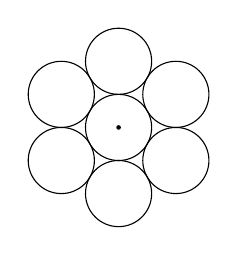
\begin{tikzpicture}[scale=0.42]
\draw (0,0) circle (1); \fill (0,0) circle (2pt);
\foreach \a in {30,90,...,330} \draw (\a:2) circle (1);
\end{tikzpicture}}\ntag{X}{}{}{}{}{parallel axis theorem}}
{\opt{$100\,mR^2$}{$55\,\dfrac{mR^2}{2}$}{$85\,\dfrac{mR^2}{2}$}{$27\,mR^2$}}

\QQ{The true length of a wire is $3.678\unit{cm}$. When the length of this wire is measured using instrument A, the length of the wire is $3.5\unit{cm}$. When the length of the wire is measured using instrument B, it is found to have length $3.38\unit{cm}$. Then the\ntag{X}{}{}{}{}{accuracy and precision of measurements}}
{\opt{measurement with A is more accurate while measurement with B is more precise.}{measurement with B is more accurate and precise.}{measurement with A is more precise while measurement with B is more accurate.}{measurement with A is more accurate and precise.}}

\QQ{A body is moving along a straight line with initial velocity $v_0$. Its acceleration $a$ is constant. After $t$ seconds, its velocity becomes $v$. The average velocity of the body over the given time interval is\ntag{A}{17}{keph102}{5}{}{Class XI Part 1 \textperiodcentered{} Ch 2}\nsrc{None found in NEET/AIPMT/AIEEE/JEE papers, 2005--2026 (NCERT concept application)}}
{\opt{$\bar v = \dfrac{v^2+v_0^2}{2at}$}{$\bar v = \dfrac{v^2+v_0^2}{at}$}{$\bar v = \dfrac{v^2-v_0^2}{2at}$}{$\bar v = \dfrac{v^2-v_0^2}{at}$}}

\QQ{A particle is in uniform circular motion. Related to one complete revolution of the particle, which among the statements is incorrect?\ntag{A}{40}{keph103}{14}{}{Class XI Part 1 \textperiodcentered{} Ch 3}\nsrc{None found in NEET/AIPMT/AIEEE/JEE papers, 2005--2026 (NCERT concept application)}}
{\opt{Displacement of the particle is zero.}{Average speed of the particle is zero.}{Average velocity of the particle is zero.}{Average acceleration of the particle is zero.}}

\QQ{$100\unit{g}$ of ice at $0^\circ$C is mixed with $100\unit{g}$ of water at $100^\circ$C. The final temperature of the mixture is [Take $L_f = 3.36\times10^5\unit{J\,kg^{-1}}$ and $S_w = 4.2\times10^3\unit{J\,kg^{-1}K^{-1}}$]\ntag{A}{209}{keph203}{8}{}{Class XI Part 2 \textperiodcentered{} Ch 10}\nsrc{None found in NEET/AIPMT/AIEEE/JEE papers, 2005--2026 (NCERT concept application)}}
{\opt{$10^\circ$C}{$50^\circ$C}{$1^\circ$C}{$40^\circ$C}}

\QQ{The P-V diagram of a Carnot's engine is shown in the graph below. The engine uses 1 mole of an ideal gas as working substance. From the graph, the area enclosed by the P-V diagram is [The heat supplied to the gas is $8000\unit{J}$]
\fig{\begin{tikzpicture}[xscale=0.5,yscale=0.72]
\draw[->] (0,0) -- (7.0,0) node[right,lbl]{$V$ (cm$^3$)};
\draw[->] (0,0) -- (0,4.6) node[above,lbl]{$P$ (kPa)};
\foreach \x in {1.25,2.5,3.75,5.0,6.25} \node[font=\tiny,below] at (\x,0) {\x};
\foreach \y/\l in {1/400,2/800,3/1200,4/1600} {\draw (0.1,\y) -- (-0.1,\y) node[left,lbl]{\l};}
\coordinate (A) at (2.5,4); \coordinate (B) at (3.75,3.2); \coordinate (C) at (6.25,1); \coordinate (D) at (2.9,2.6);
\draw[thick] (A) .. controls (3.0,3.6) .. (B) .. controls (5.0,2.0) .. (C) .. controls (4.5,1.6) .. (D) .. controls (2.6,3.1) .. (A);
\draw[densely dotted] (0,4) -- (A) -- (2.5,0) (0,3) -- (3.75,3) (B) -- (3.75,0) (D) -- (2.9,0) (0,1) -- (C) -- (6.25,0);
\node[lbl,above] at (A) {A}; \node[lbl,above right] at (B) {B}; \node[lbl,right] at (C) {C}; \node[lbl,right] at (D) {D};
\end{tikzpicture}}\ntag{A}{237}{keph204}{12}{}{Class XI Part 2 \textperiodcentered{} Ch 11}\nsrc{None found in NEET/AIPMT/AIEEE/JEE papers, 2005--2026 (NCERT concept application)}}
{\opt{$2000\unit{J}$}{$3000\unit{J}$}{$1000\unit{J}$}{$1200\unit{J}$}}

\QQ{When a planet revolves around the Sun, in general, for the planet\ntag{D}{128}{keph107}{2}{}{Class XI Part 1 \textperiodcentered{} Ch 7}}
{\opt{linear momentum and aerial velocity are constant.}{kinetic and potential energy of the planet are constant.}{angular momentum about the Sun and aerial velocity of the planet are constant.}{linear momentum and linear velocity are constant.}}

\QQ{A stretched wire of a material whose Young's modulus $Y = 2\times10^{11}\unit{N\,m^{-2}}$ has Poisson's ratio 0.25. Its lateral strain $\varepsilon_l = 10^{-3}$. The elastic energy density of the wire is\ntag{A}{174}{keph201}{8}{}{Class XI Part 2 \textperiodcentered{} Ch 8}\nsrc{None found in NEET/AIPMT/AIEEE/JEE papers, 2005--2026 (NCERT concept application)}}
{\opt{$1\times10^5\unit{J\,m^{-3}}$}{$4\times10^5\unit{J\,m^{-3}}$}{$8\times10^5\unit{J\,m^{-3}}$}{$16\times10^5\unit{J\,m^{-3}}$}}

\QQ{A closed water tank has cross-sectional area $A$. It has a small hole at a depth of $h$ from the free surface of water. The radius of the hole is $r$ so that $r\ll\sqrt{A/\pi}$. If $P_0$ is the pressure inside the tank above water level, and $P_a$ is the atmospheric pressure, the rate of flow of the water coming out of the hole is [$\rho$ is the density of water]
\fig{\begin{tikzpicture}[scale=0.7]
\draw[line width=1pt] (0,0) rectangle (2.4,2.6);
\fill[pattern=horizontal lines,pattern color=gray] (0.05,0.05) rectangle (2.35,2.1);
\draw (0.05,2.1) -- (2.35,2.1); \node[lbl] at (1.2,2.38) {$P_0$};
\draw (2.4,0.95) -- (2.75,0.95) (2.4,1.3) -- (2.75,1.3); \draw (2.75,1.125) ellipse (0.08 and 0.175);
\draw (2.83,1.2) .. controls (3.4,1.2) and (3.5,0.8) .. (3.6,0.1);
\draw[<->] (2.0,0.95) -- (2.0,1.3) node[midway,left,lbl]{$2r$};
\draw (3.9,2.1) -- (4.3,2.1) (3.9,1.125) -- (4.3,1.125) (3.9,0) -- (4.3,0);
\draw[<->] (4.1,2.1) -- (4.1,1.125) node[midway,right,lbl]{$h$};
\draw[<->] (4.1,1.125) -- (4.1,0) node[midway,right,lbl]{$H$};
\end{tikzpicture}}\ntag{A}{189}{keph202}{10}{}{Class XI Part 2 \textperiodcentered{} Ch 9}\nsrc{None found in NEET/AIPMT/AIEEE/JEE papers, 2005--2026 (NCERT concept application)}}
{\opt{$\pi r^2\sqrt{2gh+\dfrac{2(P_0-P_a)}{\rho}}$}{$\pi r^2\sqrt{2gH}$}{$\pi r^2\sqrt{gh+\dfrac{2(P_0-P_a)}{\rho}}$}{$\pi r^2\sqrt{2gh}$}}

\QQ{A positively charged glass rod is brought near uncharged metal sphere, which is mounted on an insulated stand. If the glass rod is removed, the net charge on the metal sphere is\ntag{X}{}{}{}{}{charging by induction}}
{\opt{Zero}{$1.6\times10^{-19}\unit{C}$}{Positive charge}{Negative charge}}

\QQ{In the situation shown in the diagram, magnitude of $q\ll|Q|$ and $r\gg a$. The net force on the free charge $-q$ and net torque on it about O at the instant shown are respectively [$p = 2aQ$ is the dipole moment]
\fig{\begin{tikzpicture}[scale=0.75]
\draw (-1.5,0) -- (1.5,0);
\draw[fill=parchment] (-1.5,0) circle (0.15) node{\tiny$-$}; \draw[fill=parchment] (1.5,0) circle (0.15) node{\tiny$+$};
\node[lbl,above left] at (-1.5,0.1) {A}; \node[lbl,above right] at (1.5,0.1) {B};
\node[lbl,below] at (-1.5,-0.15) {$-Q$}; \node[lbl,below] at (1.5,-0.15) {$+Q$};
\fill (0,0) circle (1.5pt) node[below,lbl]{O};
\draw[densely dashed] (0,0) -- (0,2.4); \fill (0,2.4) circle (2pt) node[left,lbl]{P} node[above,lbl]{$-q$};
\draw (0,0.2) -| (0.2,0);
\draw[|<->|] (2.0,0) -- (2.0,2.4) node[midway,right,lbl]{$r$};
\draw[|<->|] (-1.5,-0.75) -- (0,-0.75) node[midway,below,lbl]{$a$}; \draw[|<->|] (0,-0.75) -- (1.5,-0.75) node[midway,below,lbl]{$a$};
\end{tikzpicture}}\ntag{A}{23}{leph101}{23}{}{Class XII Part 1 \textperiodcentered{} Ch 1}\nsrc{None found in NEET/AIPMT/AIEEE/JEE papers, 2005--2026 (NCERT concept application)}}
{\opt{$\dfrac{1}{4\pi\varepsilon_0}\dfrac{pq}{r^2}\hat k,\ \dfrac{1}{4\pi\varepsilon_0}\dfrac{pq}{r^3}\hat i$}{$-\dfrac{1}{4\pi\varepsilon_0}\dfrac{pq}{r^2}\hat k,\ -\dfrac{1}{4\pi\varepsilon_0}\dfrac{pq}{r^3}\hat i$}{$\dfrac{1}{4\pi\varepsilon_0}\dfrac{pq}{r^3}\hat i,\ +\dfrac{1}{4\pi\varepsilon_0}\dfrac{pq}{r^2}\hat k$}{$\dfrac{1}{4\pi\varepsilon_0}\dfrac{pq}{r^3}\hat i,\ -\dfrac{1}{4\pi\varepsilon_0}\dfrac{pq}{r^2}\hat k$}}

\QQ{Pressure of ideal gas at constant volume is proportional to \rule{1.2cm}{0.4pt}.\ntag{D}{250}{keph205}{7}{}{Class XI Part 2 \textperiodcentered{} Ch 12}}
{\opt{average potential energy of the molecules}{total energy of the gas}{average kinetic energy of the molecules}{force between the molecules}}

\QQ{A block of mass $m$ is connected to a light spring of force constant $k$. The system is placed inside a damping medium of damping constant $b$. The instantaneous values of displacement, acceleration and energy of the block are $x$, $a$ and $E$ respectively. The initial amplitude of oscillation is $A$ and $\omega'$ is the angular frequency of oscillations. The incorrect expression related to the damped oscillations is\ntag{X}{}{}{}{}{damped oscillations}}
{\opt{$\omega' = \sqrt{\dfrac km-\dfrac{b^2}{4m^2}}$}{$E = \dfrac12kA^2e^{-bt/m}$}{$m\dfrac{d^2x}{dt^2}+b\dfrac{dx}{dt}+kx = 0$}{$x = Ae^{-\frac bm t}\cos(\omega't+\phi)$}}

\QQ{The speed of sound in an ideal gas at a given temperature $T$ is $v$. The rms speed of gas molecules at that temperature is $v_{rms}$. The ratio of the velocities $v$ and $v_{rms}$ for helium and oxygen gases are $X$ and $X'$ respectively. Then $\dfrac{X}{X'}$ is equal to\ntag{A}{287}{keph207}{10}{}{Class XI Part 2 \textperiodcentered{} Ch 14}\nsrc{JEE Main 2022 (25 Jul, Shift 2) -- rms speed of gas molecules compared with the speed of sound}}
{\opt{$\dfrac{5}{\sqrt{21}}$}{$\sqrt{\dfrac{5}{21}}$}{$\dfrac{21}{5}$}{$\dfrac{21}{\sqrt5}$}}

\QQ{A uniform electric field vector $\vec E$ exists along horizontal direction as shown. The electric potential at A is $V_A$. A small point charge $q$ is slowly taken from A to B along the curved path as shown. The potential energy of the charge when it is at point B is
\fig{\begin{tikzpicture}[scale=0.8]
\foreach \y in {0,0.45,0.9,1.35} \draw[densely dashed,->] (0,\y) -- (3.2,\y);
\node[lbl,right] at (3.2,0) {$\vec E$};
\fill (0.6,0.6) circle (1.5pt) node[above left,lbl]{A}; \fill (2.4,0.6) circle (1.5pt) node[above right,lbl]{B};
\draw (0.6,0.6) .. controls (0.9,0.0) and (1.3,0.4) .. (1.5,0.1) .. controls (1.8,-0.2) and (2.0,0.5) .. (2.4,0.6);
\draw (0.6,0.6) -- (0.6,1.7); \draw (2.4,0.6) -- (2.4,1.7);
\draw[<->] (0.6,1.6) -- (2.4,1.6) node[midway,above,lbl]{$x$};
\end{tikzpicture}}\ntag{A}{55}{leph102}{11}{}{Class XII Part 1 \textperiodcentered{} Ch 2}\nsrc{None found in NEET/AIPMT/AIEEE/JEE papers, 2005--2026 (NCERT concept application)}}
{\opt{$q[V_A+Ex]$}{$q[Ex-V_A]$}{$qEx$}{$q[V_A-Ex]$}}

\QQ{A parallel plate capacitor of capacitance $C_1$ with a dielectric slab in between its plates is connected to a battery. It has a potential difference $V_1$ across its plates. When the dielectric slab is removed, keeping the capacitor connected to the battery, the new capacitance and potential difference are $C_2$ and $V_2$ respectively. Then,\ntag{D}{80}{leph102}{36}{ \textperiodcentered{} Exercise 2.9}{Class XII Part 1 \textperiodcentered{} Ch 2}}
{\opt{$V_1>V_2,\ C_1>C_2$}{$V_1<V_2,\ C_1>C_2$}{$V_1=V_2,\ C_1>C_2$}{$V_1=V_2,\ C_1<C_2$}}

\QQ{A cubical Gaussian surface has side of length $a = 10\unit{cm}$. Electric field lines are parallel to $x$-axis as shown. The magnitudes of electric fields through surfaces ABCD and EFGH are $6\unit{kN\,C^{-1}}$ and $9\unit{kN\,C^{-1}}$ respectively. Then the total charge enclosed by the cube is [Take $\varepsilon_0 = 9\times10^{-12}\unit{F\,m^{-1}}$]
\fig{\begin{tikzpicture}[scale=0.85]
\coordinate (B) at (0,0); \coordinate (C) at (-0.5,-0.4); \coordinate (G) at (1.1,-0.4); \coordinate (F) at (1.6,0);
\coordinate (A) at (0,1.2); \coordinate (D) at (-0.5,0.8); \coordinate (H) at (1.1,0.8); \coordinate (E) at (1.6,1.2);
\draw (D) -- (A) -- (E) -- (H) -- cycle; \draw (D) -- (C) -- (G) -- (H); \draw (G) -- (F) -- (E);
\draw[densely dashed] (A) -- (B) -- (C) (B) -- (F);
\foreach \y in {0.15,0.45,0.75} \draw[->] (-0.9,\y) -- (2.4,\y);
\node[lbl,above] at (A) {A}; \node[lbl,below right] at (B) {B}; \node[lbl,below] at (C) {C}; \node[lbl,left] at (D) {D};
\node[lbl,above right] at (E) {E}; \node[lbl,right] at (F) {F}; \node[lbl,below] at (G) {G}; \node[lbl,above] at (H) {H};
\draw[->] (-0.6,0) -- (-0.6,1.9) node[above,lbl]{$Y$}; \node[lbl,right] at (2.4,0.15) {$X$};
\draw[->] (-0.6,0) -- (-1.2,-0.6) node[left,lbl]{$Z$};
\end{tikzpicture}}\ntag{A}{30}{leph101}{30}{}{Class XII Part 1 \textperiodcentered{} Ch 1}\nsrc{None found in NEET/AIPMT/AIEEE/JEE papers, 2005--2026 (NCERT concept application)}}
{\opt{$1.35\unit{nC}$}{$-1.35\unit{nC}$}{$0.27\unit{nC}$}{$-0.27\unit{nC}$}}

\QQ{Electric field at a distance `$r$' from an infinitely long uniformly charged straight conductor, having linear charge density $\lambda$ is $E_1$. Another uniformly charged conductor having same linear charge density $\lambda$ is bent into a semicircle of radius `$r$'. The electric field at its centre is $E_2$. Then\ntag{A}{33}{leph101}{33}{}{Class XII Part 1 \textperiodcentered{} Ch 1}\nsrc{None found in NEET/AIPMT/AIEEE/JEE papers, 2005--2026 (NCERT concept application)}}
{\opt{$E_2 = \dfrac{E_1}{r}$}{$E_1 = E_2$}{$E_1 = \pi rE_2$}{$E_2 = \pi rE_1$}}

\QQ{Five capacitors each of value $1\unit{\mu F}$ are connected as shown in the figure. The equivalent capacitance between A and B is
\fig{\begin{circuitikz}[scale=0.55,transform shape,font=\Large]
\draw (0,0) -- (6,0) (0,3) -- (6,3);
\draw (0,3) to[C,l_=$1\,\mu\mathrm F$] (0,1.5) to[C,l_=$1\,\mu\mathrm F$] (0,0);
\draw (3,3) to[C,l=$1\,\mu\mathrm F$] (3,0);
\draw (6,3) to[C,l=$1\,\mu\mathrm F$] (6,1.5) to[C,l=$1\,\mu\mathrm F$] (6,0);
\draw (0,1.5) -- (0.6,1.5) node[circ]{} node[right]{A};
\draw (6,1.5) -- (5.4,1.5) node[circ]{} node[left]{B};
\end{circuitikz}}\ntag{A}{71}{leph102}{27}{}{Class XII Part 1 \textperiodcentered{} Ch 2}\nsrc{None found in NEET/AIPMT/AIEEE/JEE papers, 2005--2026 (NCERT concept application)}}
{\opt{$1\unit{\mu F}$}{$2\unit{\mu F}$}{$5\unit{\mu F}$}{$3\unit{\mu F}$}}

\QQ{For a given electric current the drift velocity of conduction electrons in a copper wire is $v_d$ and their mobility is $\mu$. When the current is increased at constant temperature\ntag{A}{88}{leph103}{8}{}{Class XII Part 1 \textperiodcentered{} Ch 3}\nsrc{None found in NEET/AIPMT/AIEEE/JEE papers, 2005--2026 (NCERT concept application)}}
{\opt{$v_d$ remains the same, $\mu$ increases}{$v_d$ decreases, $\mu$ remains the same}{$v_d$ remains the same, $\mu$ decreases}{$v_d$ increases, $\mu$ remains the same}}

\QQ{Ten identical cells each emf $2\unit{V}$ and internal resistance $1\unit{\Omega}$ are connected in series with two cells wrongly connected. A resistor of $10\unit{\Omega}$ is connected to the combination. What is the current through the resistor?\ntag{A}{96}{leph103}{16}{}{Class XII Part 1 \textperiodcentered{} Ch 3}\nsrc{None found in NEET/AIPMT/AIEEE/JEE papers, 2005--2026 (NCERT concept application)}}
{\opt{$2.4\unit{A}$}{$0.6\unit{A}$}{$1.2\unit{A}$}{$1.8\unit{A}$}}

\QQ{The equivalent resistance between the points A and B in the following circuit is
\fig{\begin{circuitikz}[scale=0.55,transform shape,font=\Large]
\draw (0,2.4) node[circ]{} node[left]{A} to[R,l=$2\,\Omega$] (2,2.4) to[R,l=$2\,\Omega$] (4.4,2.4) to[R,l=$2\,\Omega$] (6.8,2.4);
\draw (0,0) node[circ]{} node[left]{B} to[R,l_=$2\,\Omega$] (2,0) to[R,l_=$2\,\Omega$] (4.4,0) to[R,l_=$2\,\Omega$] (6.8,0);
\draw (2,2.4) to[R,l=$2\,\Omega$] (2,0); \draw (4.4,2.4) to[R,l=$2\,\Omega$] (4.4,0); \draw (6.8,2.4) to[R,l=$2\,\Omega$] (6.8,0);
\draw[densely dotted] (6.8,2.4) -- (7.8,2.4) (6.8,0) -- (7.8,0);
\end{circuitikz}}\ntag{A}{97}{leph103}{17}{}{Class XII Part 1 \textperiodcentered{} Ch 3}\nsrc{None found in NEET/AIPMT/AIEEE/JEE papers, 2005--2026 (NCERT concept application)}}
{\opt{$5.5\unit{\Omega}$}{$0.05\unit{\Omega}$}{$5\unit{\Omega}$}{$0.5\unit{\Omega}$}}

\QQ{A charged particle is subjected to acceleration in a cyclotron as shown. The charged particle undergoes increase in its speed
\fig{\begin{tikzpicture}[scale=0.62]
\draw (-0.12,1.6) arc (90:270:1.6) -- (-0.12,1.6);
\draw (0.12,1.6) arc (90:-90:1.6) -- (0.12,1.6);
\foreach \p in {(-1.1,0.9),(-1.3,0.2),(-1.1,-0.7),(-0.6,1.25),(-0.5,-1.3),(1.1,0.9),(1.3,0.2),(1.1,-0.7),(0.6,1.25),(0.5,-1.3)} \fill \p circle (0.9pt);
\foreach \r in {0.25,0.45,0.65,0.85,1.05} {\draw (0,0) ++(90:\r) arc (90:270:\r); \draw (0,-\r) arc (-90:90:\r+0.1);}
\draw (-0.12,1.6) -- (-0.12,2.1) -- (-0.4,2.1); \draw (0.12,1.6) -- (0.12,2.1) -- (0.4,2.1);
\draw (-0.4,1.95) rectangle (0.4,2.4); \node[font=\tiny] at (0,2.18) {RFO};
\node[lbl] at (-0.55,1.8) {$D_1$}; \node[lbl] at (0.6,1.8) {$D_2$};
\draw[->] (1.15,-0.1) -- (1.15,-2.1);
\node[lbl] at (-1.3,-1.6) {$\odot\,\vec B$};
\end{tikzpicture}}\ntag{X}{}{}{}{}{cyclotron}}
{\opt{Only inside $D_2$}{Inside $D_1$, $D_2$ and the gaps}{Only inside $D_1$}{Only in the gap between $D_1$ and $D_2$}}

\QQ{The resistance of a carbon resistor is $4.7\unit{k\Omega}\pm5\%$. The colour of the third band is\ntag{X}{}{}{}{}{resistor colour code}}
{\opt{red}{violet}{orange}{gold}}

\QQ{The four bands of a colour coded resistor are of the colours gray, red, gold and gold. The value of the resistance of the resistor is\ntag{X}{}{}{}{}{resistor colour code}}
{\opt{$82\unit{\Omega}\pm10\%$}{$8.2\unit{\Omega}\pm5\%$}{$82\unit{\Omega}\pm5\%$}{$5.2\unit{\Omega}\pm5\%$}}

\QQ{A wire of resistance $R$ is connected across a cell of emf $\varepsilon$ and internal resistance $r$. The current through the circuit is $I$. In time $t$, the work done by the battery to establish the current $I$ is\ntag{D}{102}{leph103}{22}{}{Class XII Part 1 \textperiodcentered{} Ch 3}}
{\opt{$\dfrac{\varepsilon^2t}{R}$}{$IRt$}{$I^2Rt$}{$\varepsilon It$}}

\QQ{The Curie temperatures of Cobalt and iron are $1400\unit{K}$ and $1000\unit{K}$ respectively. At $T = 1600\unit{K}$, the ratio of magnetic susceptibility of Cobalt to that of iron is\ntag{X}{}{}{}{}{Curie--Weiss law}}
{\opt{3}{$\dfrac75$}{$\dfrac57$}{$\dfrac13$}}

\QQ{The torque acting on a magnetic dipole placed in uniform magnetic field is zero, when the angle between the dipole axis and the magnetic field is \rule{1.2cm}{0.4pt}.\ntag{D}{139}{leph105}{4}{}{Class XII Part 1 \textperiodcentered{} Ch 5}}
{\opt{$45^\circ$}{$60^\circ$}{$90^\circ$}{zero}}

\QQ{The horizontal component of Earth's magnetic field at a place is $3\times10^{-5}\unit{T}$. If the dip at that place is $45^\circ$, the resultant magnetic field at that place is\ntag{X}{}{}{}{}{Earth's magnetism (angle of dip)}}
{\opt{$\dfrac{3}{\sqrt2}\times10^{-5}\unit{T}$}{$\dfrac32\sqrt3\times10^{-5}\unit{T}$}{$3\sqrt2\times10^{-5}\unit{T}$}{$3\times10^{-5}\unit{T}$}}

\QQ{A proton and an alpha-particle moving with the same velocity enter a uniform magnetic field with their velocities perpendicular to the magnetic field. The ratio of radii of their circular paths is\ntag{D}{112}{leph104}{6}{}{Class XII Part 1 \textperiodcentered{} Ch 4}}
{\opt{1:4}{4:1}{1:2}{2:1}}

\QQ{A moving coil galvanometer is converted into an ammeter of range 0 to $5\unit{mA}$. The galvanometer resistance is $90\unit{\Omega}$ and the shunt resistance has a value of $10\unit{\Omega}$. If there are 50 divisions in the galvanometer-turned-ammeter on either sides of zero, its current sensitivity is\ntag{A}{131}{leph104}{25}{}{Class XII Part 1 \textperiodcentered{} Ch 4}\nsrc{NEET 2018 -- current sensitivity of a moving-coil galvanometer}}
{\opt{$1\times10^5\unit{A/div}$}{$2\times10^4\unit{A/div}$}{$1\times10^5\unit{div/A}$}{$2\times10^4\unit{div/A}$}}

\QQ{A positively charged particle of mass $m$ is passed through a velocity selector. It moves horizontally rightward without deviation along the line $y = \dfrac{2mv}{qB}$ with a speed $v$. The electric field is vertically downwards and magnetic field is into the plane of the paper. Now, the electric field is switched off at $t=0$. The angular momentum of the charged particle about origin O at $t = \dfrac{\pi m}{qB}$ is
\fig{\begin{tikzpicture}[scale=0.62]
\foreach \x in {1,2,3,4,5} \foreach \y in {-1.6,-0.8,0.8,1.6} \node[font=\scriptsize] at (\x,\y) {$\times$};
\foreach \y in {-1.6,-0.8,0.8,1.6} \node[font=\scriptsize] at (0,\y) {$\times$};
\draw[densely dashed] (0,-2.0) -- (0,2.0); \draw[->] (0,2.0) -- (0,2.3) node[right,lbl]{$y$};
\draw[densely dashed,->] (0,0) -- (5.8,0) node[right,lbl]{$x$};
\fill (0,0) circle (1.5pt) node[left,lbl]{O};
\fill (0,1.2) circle (2pt) node[left,lbl]{$q$}; \draw[->] (0.1,1.2) -- (0.8,1.2) node[right,lbl]{$\vec v$};
\draw[->] (2,0.9) -- (2,-1.1) node[right,lbl]{$\vec E$};
\node[lbl] at (3.55,-1.6) {$\otimes\vec B$};
\end{tikzpicture}}\ntag{X}{}{}{}{}{velocity selector}}
{\opt{$\dfrac{2mE^2}{qB^3}$}{zero}{$\dfrac{mE^3}{qB^2}$}{$\dfrac{mE^2}{qB^3}$}}

\QQ{In series LCR circuit at resonance, the phase difference between voltage and current is\ntag{D}{191}{leph107}{15}{}{Class XII Part 1 \textperiodcentered{} Ch 7}}
{\opt{$\pi$}{$\dfrac\pi4$}{$\dfrac\pi2$}{zero}}

\QQ{An ideal transformer has a turns ratio of 10. When the primary is connected to $220\unit{V}$, $50\unit{Hz}$ ac source, the power output is\ntag{D}{195}{leph107}{19}{}{Class XII Part 1 \textperiodcentered{} Ch 7}}
{\opt{$\frac{1}{10}$th the power input}{equal to power input}{zero}{10 times the power input}}

\QQ{The current in a coil changes from $2\unit{A}$ to $5\unit{A}$ in $0.3\unit{s}$. The magnitude of emf induced in the coil is $1.0\unit{V}$. The value of self-inductance of the coil is\ntag{D}{176}{leph106}{23}{ \textperiodcentered{} Exercise 6.7}{Class XII Part 1 \textperiodcentered{} Ch 6}}
{\opt{$100\unit{mH}$}{$0.1\unit{mH}$}{$10\unit{mH}$}{$1.0\unit{mH}$}}

\QQ{A metallic rod of length $1\unit{m}$ held along east-west direction is allowed to fall down freely. Given horizontal component of earth's magnetic field $B_H = 3\times10^{-5}\unit{T}$. The emf induced in the rod at an instant $t = 2\unit{s}$ after it is released is (Take $g = 10\unit{m\,s^{-2}}$)\ntag{D}{176}{leph106}{23}{ \textperiodcentered{} Exercise 6.6}{Class XII Part 1 \textperiodcentered{} Ch 6}}
{\opt{$3\times10^{-3}\unit{V}$}{$3\times10^{-4}\unit{V}$}{$6\times10^{-3}\unit{V}$}{$6\times10^{-4}\unit{V}$}}

\QQ{A square loop of side $2\unit{cm}$ enters a magnetic field with a constant speed of $2\unit{cm\,s^{-1}}$ as shown. The front edge enters the field at $t = 0\unit{s}$. Which of the following graph correctly depicts the induced emf in the loop? (Take clockwise direction positive)
\fig{\begin{tikzpicture}[scale=0.55]
\draw (0,0) rectangle (1.6,1.6); \node[lbl,above] at (0.8,1.6) {2 cm}; \draw[->] (1.6,0.8) -- (2.4,0.8);
\foreach \x in {2.1,3.0,3.9} \foreach \y in {-0.6,0.1,0.8,1.5,2.2} \node[font=\scriptsize] at (\x,\y) {$\times$};
\node[lbl,right] at (4.1,0.8) {$B = 0.5\unit{T}$};
\draw[<->] (2.1,-1.1) -- (3.9,-1.1) node[midway,below,lbl]{10 cm};
\end{tikzpicture}}\ntag{A}{163}{leph106}{10}{}{Class XII Part 1 \textperiodcentered{} Ch 6}\nsrc{JEE Main 2024 (9 Apr, Shift 2) -- square loop entering a magnetic field at constant speed, induced emf}}
{\optfig{\emfg{\draw (0,0) -- (0,1) -- (1,0) -- (5,0) -- (5,-1) -- (6,0);}}
{\emfg{\draw (0,0) -- (0,-1) -- (1,0) -- (5,0) -- (5,1) -- (6,0);}}
{\emfg{\draw (0,0) -- (0,-1) -- (1,-1) -- (1,0) -- (5,0) -- (5,1) -- (6,1) -- (6,0);}}
{\emfg{\draw (0,0) -- (0,1) -- (1,1) -- (1,0) -- (5,0) -- (5,-1) -- (6,-1) -- (6,0);}}}

\QQ{For a given pair of transparent media, the critical angle for which colour is maximum?\ntag{A}{230}{leph201}{10}{}{Class XII Part 2 \textperiodcentered{} Ch 9}\nsrc{None found in NEET/AIPMT/AIEEE/JEE papers, 2005--2026 (NCERT concept application)}}
{\opt{Red}{Blue}{Violet}{Green}}

\QQ{An equiconvex lens made of glass of refractive index $\frac32$ has focal length $f$ in air. It is completely immersed in water of refractive index $\frac43$. The percentage change in the focal length is\ntag{D}{237}{leph201}{17}{ \textperiodcentered{} Example 9.7}{Class XII Part 2 \textperiodcentered{} Ch 9}}
{\opt{300\% decrease}{400\% decrease}{300\% increase}{400\% increase}}

\QQ{A point object is moving at a constant speed of $1\unit{m\,s^{-1}}$ along the principal axis of a convex lens of focal length $10\unit{cm}$. The speed of the image is also $1\unit{m\,s^{-1}}$, when the object is at \rule{1cm}{0.4pt} cm from the optic centre of the lens.\ntag{A}{236}{leph201}{16}{}{Class XII Part 2 \textperiodcentered{} Ch 9}\nsrc{None found in NEET/AIPMT/AIEEE/JEE papers, 2005--2026 (NCERT concept application)}}
{\opt{15}{20}{5}{10}}

\QQ{When light propagates through a given homogeneous medium, the velocities of\ntag{D}{257}{leph202}{3}{}{Class XII Part 2 \textperiodcentered{} Ch 10}}
{\opt{primary wavefronts are lesser than those of secondary wavelets.}{primary wavefronts are greater than or equal to those of secondary wavelets.}{primary wavefront and wavelets are equal.}{primary wavefront are larger than those of secondary wavelets.}}

\QQ{Total impedance of a series LCR circuit varies with angular frequency of the AC source connected to it as shown in the graph. The quality factor Q of the series LCR circuit is
\fig{\begin{tikzpicture}[xscale=0.62,yscale=0.8]
\draw[->] (0,0) -- (7.2,0) node[right,lbl]{$\omega$ (rad\,s$^{-1}$)};
\draw[->] (0,0) -- (0,2.6) node[above,lbl]{$Z$ ($\Omega$)};
\foreach \x in {1,...,6} {\draw (\x,0.05) -- (\x,-0.05); \node[font=\tiny,below] at (\x,0) {\x00};}
\draw[densely dashed] (0,1.0) node[left,lbl]{$Z_{min}$} -- (6.6,1.0);
\draw[densely dashed] (0,1.414) node[left,lbl]{$\sqrt2Z_{min}$} -- (6.6,1.414);
\draw[densely dashed] (4,1.414) -- (4,0) (5,1.0) -- (5,0) (6,1.414) -- (6,0);
\draw[domain=2.8:7.0,samples=60] plot (\x,{sqrt(1+(\x-5)^2)});
\end{tikzpicture}}\ntag{X}{}{}{}{}{sharpness (quality factor) of resonance}}
{\opt{2.5}{5}{1}{0.4}}

\QQ{The ratio of the magnitudes of electric field to the magnetic field of an electromagnetic wave is of the order of\ntag{D}{207}{leph108}{7}{}{Class XII Part 1 \textperiodcentered{} Ch 8}}
{\opt{$10^5\unit{m\,s^{-1}}$}{$10^{-5}\unit{m\,s^{-1}}$}{$10^8\unit{m\,s^{-1}}$}{$10^{-8}\unit{m\,s^{-1}}$}}

\QQ{For a point object, which of the following always produces virtual image in air?\ntag{D}{249}{leph201}{29}{ \textperiodcentered{} Exercise 9.15}{Class XII Part 2 \textperiodcentered{} Ch 9}}
{\opt{Plano-convex lens}{Convex mirror}{Biconvex lens}{Concave mirror}}

\QQ{In an experiment to study photo-electric effect the observed variation of stopping potential with frequency of incident radiation is as shown in the figure. The slope and $y$-intercept are respectively ($V_0$: stopping potential; $\nu$: frequency of incident radiation)
\fig{\begin{tikzpicture}[scale=0.8]
\draw[->] (-0.2,0) -- (3.2,0) node[right,lbl]{$\nu$};
\draw[->] (0,-0.3) -- (0,2.4) node[above,lbl]{$V_0$};
\draw (1.0,0) -- (2.0,2.1); \node[lbl,below] at (1.0,0) {$\nu_0$};
\end{tikzpicture}}\ntag{D}{282}{leph203}{9}{}{Class XII Part 2 \textperiodcentered{} Ch 11}}
{\opt{$\dfrac{h\nu}{e},\ \nu_0$}{$\dfrac{h\nu}{e},\ -\dfrac he$}{$h\nu,\ -h\nu_0$}{$\dfrac he,\ -\dfrac{h\nu_0}{e}$}}

\QQ{In the Rutherford's alpha scattering experiment, as the impact parameter increases, the scattering angle of the alpha particle\ntag{D}{294}{leph204}{5}{}{Class XII Part 2 \textperiodcentered{} Ch 12}}
{\opt{is always $90^\circ$}{decreases}{increases}{remains the same}}

\QQ{Three energy levels of hydrogen atom and the corresponding wavelength of the emitted radiation due to different electron transition are as shown. Then
\fig{\begin{tikzpicture}[scale=0.8]
\draw (0,0) -- (3.6,0) node[right,lbl]{$E_1$}; \draw (0,1.1) -- (3.6,1.1) node[right,lbl]{$E_2$}; \draw (0,1.7) -- (3.6,1.7) node[right,lbl]{$E_3$};
\draw[->] (0.4,1.1) -- (0.4,0) node[midway,right,lbl]{$\lambda_1$};
\draw[->] (1.8,1.7) -- (1.8,0) node[midway,right,lbl]{$\lambda_2$};
\draw[->] (2.9,1.7) -- (2.9,1.1) node[midway,left,lbl]{$\lambda_3$};
\end{tikzpicture}}\ntag{A}{300}{leph204}{11}{}{Class XII Part 2 \textperiodcentered{} Ch 12}\nsrc{AIPMT 2005 (Prelims) -- energy levels A, B, C and the wavelengths of the transitions}}
{\opt{$\lambda_1 = \dfrac{\lambda_2\lambda_3}{\lambda_2+\lambda_3}$}{$\lambda_2 = \lambda_1+\lambda_3$}{$\lambda_2 = \dfrac{\lambda_1\lambda_3}{\lambda_1+\lambda_3}$}{$\lambda_3 = \dfrac{\lambda_1\lambda_2}{\lambda_1+\lambda_2}$}}

\QQ{An unpolarised light of intensity $I$ is passed through two polaroids kept one after the other with their planes parallel to each other. The intensity of light emerging from second polaroid is $\dfrac I4$. The angle between the pass axes of the polaroids is\ntag{D}{270}{leph202}{16}{}{Class XII Part 2 \textperiodcentered{} Ch 10}}
{\opt{$0^\circ$}{$60^\circ$}{$30^\circ$}{$45^\circ$}}

\QQ{In the Young's double slit experiment, the intensity of light passing through each of the two double slits is $2\times10^{-2}\unit{W\,m^{-2}}$. The screen-slit distance is very large in comparison with slit-slit distance. The fringe width is $\beta$. The distance between the central maximum and a point P on the screen is $x = \dfrac\beta3$. Then the total light intensity at that point is\ntag{A}{264}{leph202}{10}{}{Class XII Part 2 \textperiodcentered{} Ch 10}\nsrc{None found in NEET/AIPMT/AIEEE/JEE papers, 2005--2026 (NCERT concept application)}}
{\opt{$4\times10^{-2}\unit{W\,m^{-2}}$}{$2\times10^{-2}\unit{W\,m^{-2}}$}{$16\times10^{-2}\unit{W\,m^{-2}}$}{$8\times10^{-2}\unit{W\,m^{-2}}$}}

\QQ{A $60\unit{W}$ source emits monochromatic light of wavelength $662.5\unit{nm}$. The number of photons emitted per second is\ntag{D}{284}{leph203}{11}{ \textperiodcentered{} Example 11.1}{Class XII Part 2 \textperiodcentered{} Ch 11}}
{\opt{$2\times10^{20}$}{$5\times10^{26}$}{$2\times10^{29}$}{$5\times10^{17}$}}

%%BEGIN-ANALYSIS
\end{multicols}
\par\needspace{16\baselineskip}\vspace{14pt}
\begin{center}{\pgfornament[width=3.2cm,color=gilt]{87}}\par
{\large\color{navy}\scshape KCET 2023 \textperiodcentered{} Answer Key}\end{center}
{\small\setlength{\tabcolsep}{1pt}\renewcommand{\arraystretch}{1.5}
\begin{tabularx}{\linewidth}{@{}*{10}{>{\centering\arraybackslash}X}@{}}\toprule
\textbf{1}\,(D) & \textbf{2}\,(C) & \textcolor{gray}{\textbf{3}\,(B)$^{\dagger}$} & \textcolor{gray}{\textbf{4}\,(D)$^{\dagger}$} & \textcolor{gray}{\textbf{5}\,(D)$^{\dagger}$} & \textcolor{gray}{\textbf{6}\,(A)$^{\dagger}$} & \textcolor{gray}{\textbf{7}\,(A)$^{\dagger}$} & \textbf{8}\,(D) & \textbf{9}\,(A) & \textbf{10}\,(B)\\
\textcolor{gray}{\textbf{11}\,(D)$^{*}$$^{\dagger}$} & \textcolor{gray}{\textbf{12}\,(A)$^{\dagger}$} & \textbf{13}\,(C) & \textbf{14}\,(B) & \textbf{15}\,(A) & \textbf{16}\,(B)$^{*}$ & \textbf{17}\,(C) & \textbf{18}\,(D) & \textbf{19}\,(A) & \textcolor{gray}{\textbf{20}\,(A)$^{\dagger}$}\\
\textbf{21}\,(D) & \textbf{22}\,(C) & \textcolor{gray}{\textbf{23}\,(D)$^{\dagger}$} & \textbf{24}\,(A) & \textbf{25}\,(D) & \textbf{26}\,(C) & \textbf{27}\,(C) & \textbf{28}\,(B) & \textbf{29}\,(A) & \textbf{30}\,(D)\\
\textbf{31}\,(B) & \textbf{32}\,(A)$^{*}$ & \textcolor{gray}{\textbf{33}\,(D)$^{\dagger}$} & \textcolor{gray}{\textbf{34}\,(A)$^{\dagger}$} & \textcolor{gray}{\textbf{35}\,(B)$^{\dagger}$} & \textbf{36}\,(D) & \textcolor{gray}{\textbf{37}\,(A)$^{\dagger}$} & \textbf{38}\,(D) & \textcolor{gray}{\textbf{39}\,(C)$^{\dagger}$} & \textbf{40}\,(C)\\
\textbf{41}\,(C)$^{*}$ & \textcolor{gray}{\textbf{42}\,--$^{*}$$^{\dagger}$} & \textbf{43}\,(D) & \textbf{44}\,(B) & \textbf{45}\,(A) & \textbf{46}\,(D) & \textbf{47}\,(C) & \textbf{48}\,(A) & \textbf{49}\,(C) & \textbf{50}\,(B)\\
\textbf{51}\,(C) & \textcolor{gray}{\textbf{52}\,(A)$^{\dagger}$} & \textbf{53}\,(C) & \textbf{54}\,(B) & \textbf{55}\,(D) & \textbf{56}\,(B) & \textbf{57}\,(C) & \textbf{58}\,(D) & \textbf{59}\,(B) & \textbf{60}\,(A)\\\bottomrule\end{tabularx}}\par\smallskip
{\footnotesize Answers solved by the editor; (A)--(D) are the printed options. {\color{gray}Grey$^{\dagger}$}: deleted portion (answer given for completeness). --: no option is correct. $^{*}$: see note.\par
\par\smallskip\textbf{Q11.} Taken literally (six outer discs): $27mR^2$. If all seven discs are meant: $55mR^2/2$, option (B).
\par\smallskip\textbf{Q16.} Efficiency $= 1 - 2.5/4 = 0.375$ from $PV$ of the two isotherms.
\par\smallskip\textbf{Q32.} Infinite ladder: $R = 2 + \sqrt{12} = 5.46\,\Omega$.
\par\smallskip\textbf{Q41.} Galvanometer current at full scale is 0.5\,mA for 50 divisions.
\par\smallskip\textbf{Q42.} None of the options is dimensionally correct (each lacks a factor of $m$).
}\par
\clearpage
\begin{center}{\pgfornament[width=5cm,color=gilt]{87}}\par
{\fontsize{20}{24}\selectfont\color{navy}\scshape KCET 2023 \textperiodcentered{} Paper Analysis}\par
{\color{gilt}\pgfornament[width=5cm,color=gilt,symmetry=h]{87}}\end{center}
\vspace{4pt}
\begin{multicols}{2}
\textbf{\color{crimson}1. Direct vs Applied}\par\smallskip
{\footnotesize Checked question by question against the four 2026-27 NCERT books (XI Part 1 \& 2, XII Part 1 \& 2). Out of 60, 44 questions are in the present syllabus; percentages are of these.}\par\smallskip
\begin{tabular}{@{}lrr@{}}\toprule
Direct from NCERT & \textbf{20} & 45\%\\
\quad text, summary, table or figure & 14 &\\
\quad NCERT solved Example & 2 &\\
\quad NCERT Exercise & 4 &\\
Applied (concept in NCERT) & \textbf{24} & 55\%\\\midrule
Analysed & 44 &\\
Deleted portion (not analysed) & 16 &\\\midrule
\textbf{Total} & \textbf{60} &\\\bottomrule\end{tabular}\par\smallskip
{\footnotesize Direct: Q 2, 10, 17, 22, 26, 36, 38, 40, 43, 44, 45, 46, 49, 51, 53, 54, 55, 56, 58, 60.\\ From NCERT Examples: Q 49 (Example 9.7), 60 (Example 11.1).\\ From NCERT Exercises: Q 26 (Exercise 2.9), 45 (Exercise 6.7), 46 (Exercise 6.6), 54 (Exercise 9.15).}\par\medskip
\textbf{\color{crimson}2. Where the applied questions resemble earlier exams}\par\smallskip
Of the 24 applied questions, \textbf{5} closely resemble a question from an earlier national exam:
NEET/AIPMT/AIIMS 3, JEE Main/Advanced 2, AIEEE 0. The other 19 (Q 1, 8, 13, 14, 15, 16, 18, 19, 21, 25, 27, 28, 29, 30, 31, 32, 48, 50, 59) had no close match in the NEET, AIPMT, AIIMS, AIEEE and JEE papers of 2005--2026 that were searched; they are straightforward applications of NCERT concepts.\par
{\footnotesize Strongest repeats: Q9 (AIPMT 2015), Q57 (AIPMT 2005), Q47 (JEE Main 2024).}\par\medskip
\textbf{\color{crimson}3. Difficulty level}\par\smallskip
\begin{tabular}{@{}lr@{}}\toprule
Easy & 24\\ Moderate & 19\\ Hard & 1\\\bottomrule\end{tabular}\par\smallskip
{\footnotesize Hard: Q 21. Overall: \textbf{moderate}, harder than 2024; Q11 (seven discs), Q21 (force and torque from a dipole) and Q42 (particle after the electric field is switched off) need several steps. Class XI: 12 questions, Class XII: 32 (analysed questions only). (Difficulty is the editor's assessment.)}\par\medskip
\columnbreak
\textbf{\color{crimson}4. Chapter-wise distribution}\par\smallskip
{\footnotesize\begin{tabular}{@{}p{4.7cm}c@{\,}r@{\,}r@{\,}r@{}}\toprule
Chapter & Cl. & Qs & Dir & App\\\midrule
Motion in a Straight Line & XI & 1 & 0 & 1\\
Motion in a Plane & XI & 1 & 0 & 1\\
Laws of Motion & XI & 1 & 0 & 1\\
Work, Energy \& Power & XI & 1 & 0 & 1\\
Rotational Motion & XI & 1 & 1 & 0\\
Gravitation & XI & 1 & 1 & 0\\
Mech.\ Prop.\ of Solids & XI & 1 & 0 & 1\\
Mech.\ Prop.\ of Fluids & XI & 1 & 0 & 1\\
Thermal Prop.\ of Matter & XI & 1 & 0 & 1\\
Thermodynamics & XI & 1 & 0 & 1\\
Kinetic Theory & XI & 1 & 1 & 0\\
Waves & XI & 1 & 0 & 1\\
Electric Charges \& Fields & XII & 3 & 0 & 3\\
Electrostatic Potential \& Capacitance & XII & 3 & 1 & 2\\
Current Electricity & XII & 4 & 1 & 3\\
Moving Charges \& Magnetism & XII & 2 & 1 & 1\\
Magnetism \& Matter & XII & 1 & 1 & 0\\
Electromagnetic Induction & XII & 3 & 2 & 1\\
Alternating Current & XII & 2 & 2 & 0\\
Electromagnetic Waves & XII & 1 & 1 & 0\\
Ray Optics & XII & 4 & 2 & 2\\
Wave Optics & XII & 3 & 2 & 1\\
Dual Nature & XII & 2 & 2 & 0\\
Atoms & XII & 2 & 1 & 1\\
Semiconductor Electronics & XII & 2 & 1 & 1\\
\bottomrule\end{tabular}}\par\medskip
\textbf{\color{crimson}5. Teaching takeaways}\par\smallskip
{\footnotesize\begin{itemize}[leftmargin=1em,nosep]
\item NCERT text asked directly: Kepler's second law (p.\,128), pressure and mean kinetic energy (p.\,250), Huygens' secondary wavelets (p.\,257), impact parameter (p.\,294), $V_0$--$\nu$ graph (p.\,282).
\item Solved Examples repeated: Example 9.7 (lens immersed in water), Example 11.1 (photons emitted per second).
\item Exercises repeated: Exercise 2.9 (dielectric slab with battery connected), Exercise 6.6 (falling horizontal rod), Exercise 6.7 (self-inductance from emf), Exercise 9.15 (convex mirror always forms a virtual image).
\item Sixteen questions are on deleted portions (logic gates, LED, decay, parallel-axis theorem, accuracy and precision, induction, damped oscillations, cyclotron, colour code, Curie--Weiss law, dip, velocity selector, $Q$-factor); KCET 2023 still followed the older syllabus for these.
\end{itemize}}\par\medskip
\textbf{\color{crimson}6. Deleted portions}\par\smallskip
\textbf{16} of the 60 questions are on topics removed from the 2026-27 NCERT (rationalised syllabus). They are marked \textsc{Deleted Portion} and are not analysed: digital electronics (logic gates) (Q 3); light-emitting diode (Q 4); beta-decay (Q 5); alpha-decay (Q 6); radioactive decay law (half-life) (Q 7); parallel axis theorem (Q 11); accuracy and precision of measurements (Q 12); charging by induction (Q 20); damped oscillations (Q 23); cyclotron (Q 33); resistor colour code (Q 34, 35); Curie--Weiss law (Q 37); Earth's magnetism (angle of dip) (Q 39); velocity selector (Q 42); sharpness (quality factor) of resonance (Q 52).\par
\end{multicols}
%%END-ANALYSIS









